\documentclass[]{article}
\usepackage{lmodern}
\usepackage{amssymb,amsmath}
\usepackage{ifxetex,ifluatex}
\usepackage{fixltx2e} % provides \textsubscript
\ifnum 0\ifxetex 1\fi\ifluatex 1\fi=0 % if pdftex
  \usepackage[T1]{fontenc}
  \usepackage[utf8]{inputenc}
\else % if luatex or xelatex
  \ifxetex
    \usepackage{mathspec}
  \else
    \usepackage{fontspec}
  \fi
  \defaultfontfeatures{Ligatures=TeX,Scale=MatchLowercase}
\fi
% use upquote if available, for straight quotes in verbatim environments
\IfFileExists{upquote.sty}{\usepackage{upquote}}{}
% use microtype if available
\IfFileExists{microtype.sty}{%
\usepackage{microtype}
\UseMicrotypeSet[protrusion]{basicmath} % disable protrusion for tt fonts
}{}
\usepackage[margin=1in]{geometry}
\usepackage{hyperref}
\hypersetup{unicode=true,
            pdftitle={Appendix 2: Shiny Application},
            pdfauthor={Daniël Lakens \& Aaron R. Caldwell},
            pdfborder={0 0 0},
            breaklinks=true}
\urlstyle{same}  % don't use monospace font for urls
\usepackage{graphicx,grffile}
\makeatletter
\def\maxwidth{\ifdim\Gin@nat@width>\linewidth\linewidth\else\Gin@nat@width\fi}
\def\maxheight{\ifdim\Gin@nat@height>\textheight\textheight\else\Gin@nat@height\fi}
\makeatother
% Scale images if necessary, so that they will not overflow the page
% margins by default, and it is still possible to overwrite the defaults
% using explicit options in \includegraphics[width, height, ...]{}
\setkeys{Gin}{width=\maxwidth,height=\maxheight,keepaspectratio}
\IfFileExists{parskip.sty}{%
\usepackage{parskip}
}{% else
\setlength{\parindent}{0pt}
\setlength{\parskip}{6pt plus 2pt minus 1pt}
}
\setlength{\emergencystretch}{3em}  % prevent overfull lines
\providecommand{\tightlist}{%
  \setlength{\itemsep}{0pt}\setlength{\parskip}{0pt}}
\setcounter{secnumdepth}{0}
% Redefines (sub)paragraphs to behave more like sections
\ifx\paragraph\undefined\else
\let\oldparagraph\paragraph
\renewcommand{\paragraph}[1]{\oldparagraph{#1}\mbox{}}
\fi
\ifx\subparagraph\undefined\else
\let\oldsubparagraph\subparagraph
\renewcommand{\subparagraph}[1]{\oldsubparagraph{#1}\mbox{}}
\fi

%%% Use protect on footnotes to avoid problems with footnotes in titles
\let\rmarkdownfootnote\footnote%
\def\footnote{\protect\rmarkdownfootnote}

%%% Change title format to be more compact
\usepackage{titling}

% Create subtitle command for use in maketitle
\providecommand{\subtitle}[1]{
  \posttitle{
    \begin{center}\large#1\end{center}
    }
}

\setlength{\droptitle}{-2em}

  \title{Appendix 2: Shiny Application}
    \pretitle{\vspace{\droptitle}\centering\huge}
  \posttitle{\par}
  \subtitle{Manuscript: Simulation-Based Power-Analysis for Factorial ANOVA Designs}
  \author{Daniël Lakens \& Aaron R. Caldwell}
    \preauthor{\centering\large\emph}
  \postauthor{\par}
    \date{}
    \predate{}\postdate{}
  

\begin{document}
\maketitle

The goal of ANOVApower is to easily simulate ANOVA designs and calculate
the observed power. However, we recognize that many people do not have
experience using the R programming langauge. Therefore, we developed a
``Shiny'' application (\url{http://shiny.ieis.tue.nl/anova_power/})
which provides a web-based graphical user interface for the R functions.
In the manuscript we referenced numerous simulations, and within this
appendix we have reproduced these simulations using the ANOVApower Shiny
App.

\subsection{Design Input}\label{design-input}

The Shiny App can create designs up three factors, for both within,
between, and mixed designs. It requires the following input: design
string, factor labels, sample size per cell, standard deviation,
correlation for within-subjects factors, a vector of means, adjustment
for multiple comparisons, and set the seed number.

For the design string element, Add numbers for each factor that specify
the number of levels in the factors (e.g., 2 for a factor with 2
levels). Add a `w' after the number for within-subjects factors, and a
`b' for between-subjects factors. Seperate factors with asterisks. Thus
'2b*3w' is a design with two factors, the first of which has 2 between
levels, and the second of which has 3 within levels.

\begin{figure}
\centering
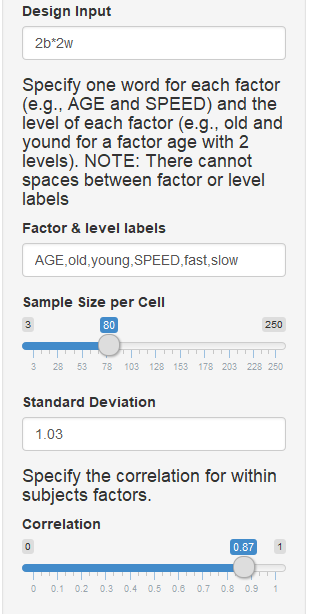
\includegraphics{https://raw.githubusercontent.com/Lakens/ANOVA_power_simulation/master/Appendix/DataEntry.PNG}
\caption{Initial Input}
\end{figure}

\begin{figure}
\centering
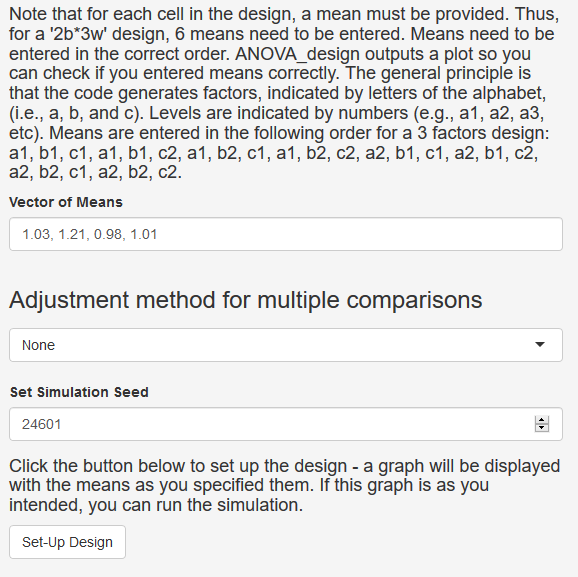
\includegraphics{https://raw.githubusercontent.com/Lakens/ANOVA_power_simulation/master/Appendix/DataEntry2.PNG}
\caption{Initial Input, cont.}
\end{figure}

\subsection{Simulation Input}\label{simulation-input}

A few more items need to be input for the simulation to run: the alpha
level and number of simulations.

\begin{figure}
\centering
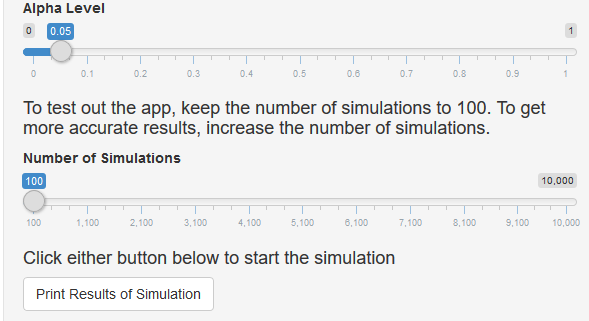
\includegraphics{https://raw.githubusercontent.com/Lakens/ANOVA_power_simulation/master/Appendix/ANOVApowerInput.PNG}
\caption{Simulation Input}
\end{figure}

\subsection{Settings from the
manuscript}\label{settings-from-the-manuscript}

In order to reproduce the simulations from the manuscript we need to set
the seed number to 2019 for \textbf{each} simulation.

\begin{figure}
\centering
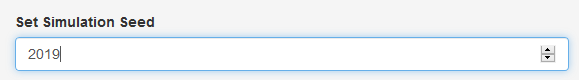
\includegraphics{https://raw.githubusercontent.com/Lakens/ANOVA_power_simulation/master/Appendix/2019_set_seed.PNG}
\caption{}
\end{figure}

The simulation reptitions should be set to 100000, but the Shiny app has
a maximum of 10000. So, for the sake of this example we will set the
number of simulations to 10000.

\begin{figure}
\centering
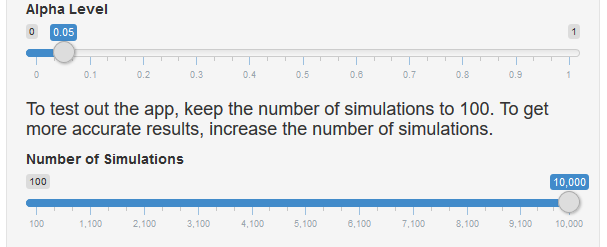
\includegraphics{https://raw.githubusercontent.com/Lakens/ANOVA_power_simulation/master/Appendix/Num_Simulations.PNG}
\caption{}
\end{figure}

\section{Simple 2 group between-subjects
design}\label{simple-2-group-between-subjects-design}

The initial study from the manuscript described a study wherein
participants interact with an artificial voice assistant who sounds
either cheerful or sad, and enjoyment is measured on scale (-5 to +5).

First, we need to set the ``Design Input'' to a two-level
between-participant design (``2b'').

\begin{figure}
\centering
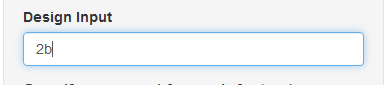
\includegraphics{https://raw.githubusercontent.com/Lakens/ANOVA_power_simulation/master/Appendix/DesignInput_2bSim.PNG}
\caption{}
\end{figure}

Next, we need to specifiy factor and level labels.

\begin{figure}
\centering
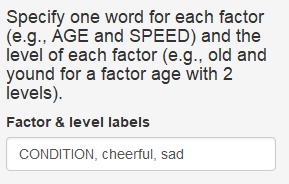
\includegraphics{https://raw.githubusercontent.com/Lakens/ANOVA_power_simulation/master/Appendix/FactorLabels_2bSim.PNG}
\caption{}
\end{figure}

The ``standard Deviation'' and ``Sample Size per Cell'' can now be set
to 2.0 and 80 respectively. Since there are no between subjects factors,
we can ignore the correlation.

\begin{figure}
\centering
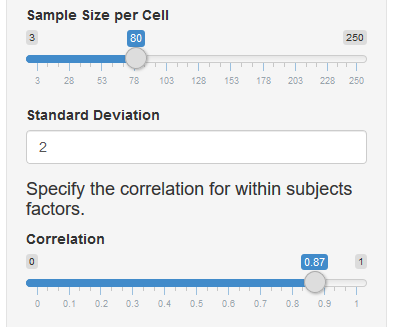
\includegraphics{https://raw.githubusercontent.com/Lakens/ANOVA_power_simulation/master/Appendix/SizeSDCorr_2bSim.PNG}
\caption{}
\end{figure}

We now enter the vector of means corresponding to the current design.

\begin{figure}
\centering
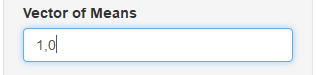
\includegraphics{https://raw.githubusercontent.com/Lakens/ANOVA_power_simulation/master/Appendix/Means_2bSim.PNG}
\caption{}
\end{figure}

Now, we can click the ``Set-Up Design'' button.

And we can check the output to ensure the design is entered correctly.

\begin{figure}
\centering
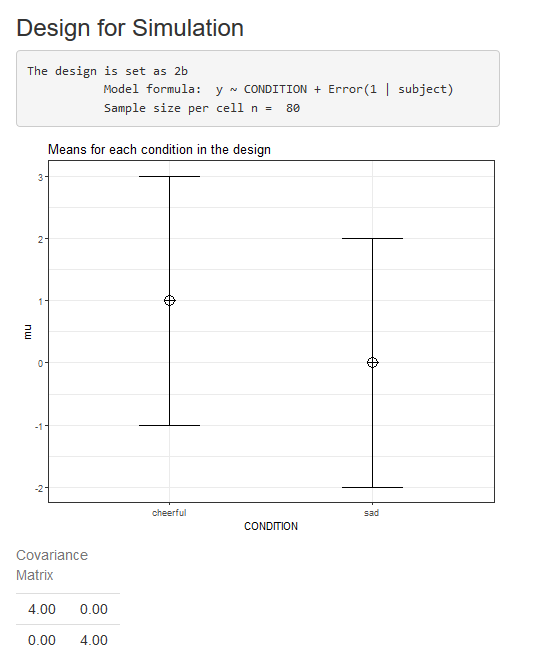
\includegraphics{https://raw.githubusercontent.com/Lakens/ANOVA_power_simulation/master/Appendix/DesignOutput_2bSim.PNG}
\caption{}
\end{figure}

The output is correct, so we can check the simulation settings then
click ``Print Results of Simulation''

\begin{figure}
\centering
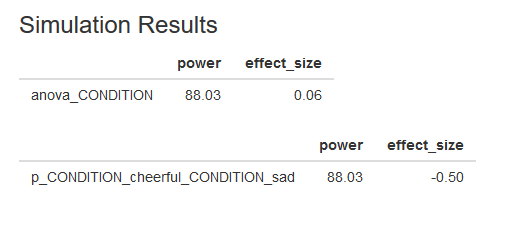
\includegraphics{https://raw.githubusercontent.com/Lakens/ANOVA_power_simulation/master/Appendix/SimResult_2bSim.PNG}
\caption{}
\end{figure}

We can also download a Markdown report of the simulation results by
clicking the ``Download Report'' button.

\begin{figure}
\centering
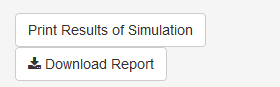
\includegraphics{https://raw.githubusercontent.com/Lakens/ANOVA_power_simulation/master/Appendix/DownloadReport.PNG}
\caption{}
\end{figure}

You can find the Markdown report from this ``2b'' simulation
\href{https://github.com/Lakens/ANOVA_power_simulation/blob/master/Appendix/Report_2bSim.pdf}{here}.

\subsection{Extending to 3 conditions}\label{extending-to-3-conditions}

In the next example, we explored what would happen if we extended the
design to 3 between-participant conditions. This was accomplished by
adding a ``neutral'' condition. Make sure the labels and mean correspond
when specifying the design.

\begin{figure}
\centering
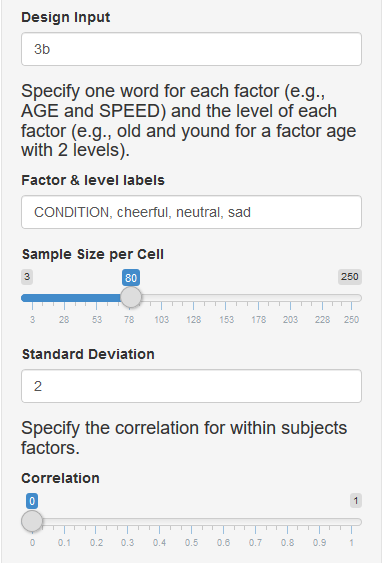
\includegraphics{https://raw.githubusercontent.com/Lakens/ANOVA_power_simulation/master/Appendix/DesignInput1_3b1Sim.PNG}
\caption{}
\end{figure}

In this scenario, the expected means were 1 (cheerful), 0.5 (neutral),
and 0 (sad).

\begin{figure}
\centering
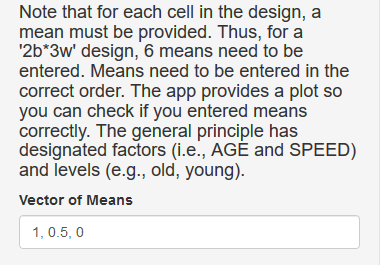
\includegraphics{https://raw.githubusercontent.com/Lakens/ANOVA_power_simulation/master/Appendix/DesignInput2_3b1Sim.PNG}
\caption{}
\end{figure}

We again check the design output to ensure the design is correct.

\begin{figure}
\centering
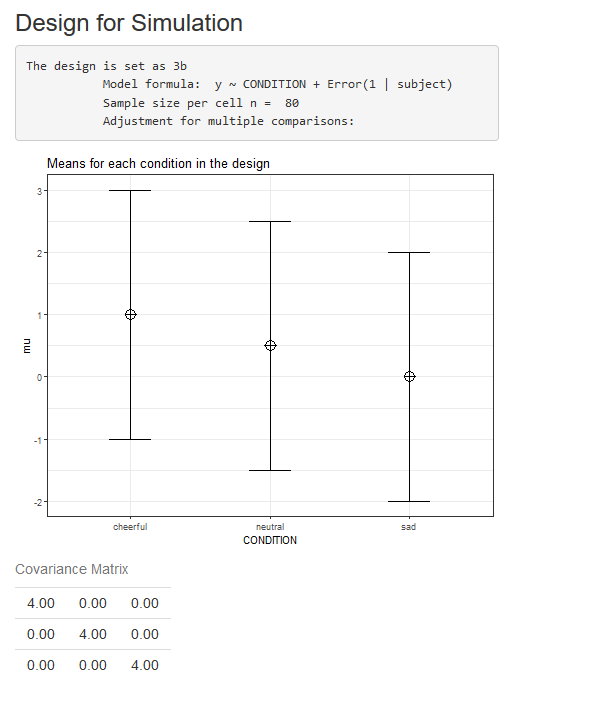
\includegraphics{https://raw.githubusercontent.com/Lakens/ANOVA_power_simulation/master/Appendix/DesignOutput_3b1Sim.PNG}
\caption{}
\end{figure}

Now we can simulate this design by clicking the ``Print Results of
Simulation'' button. The results should match the image below.

\begin{figure}
\centering
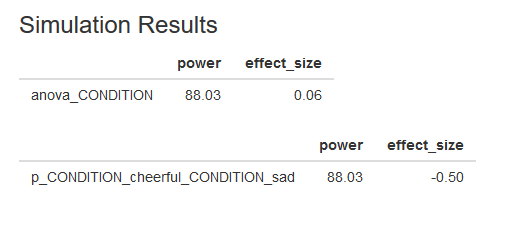
\includegraphics{https://raw.githubusercontent.com/Lakens/ANOVA_power_simulation/master/Appendix/SimResult_2bSim.PNG}
\caption{}
\end{figure}

Again, we can download a Markdown report of the results which can be
found
\href{https://github.com/Lakens/ANOVA_power_simulation/blob/master/Appendix/Report_3b1Sim.pdf}{here}.

\section{Changing to a within-subjects
design}\label{changing-to-a-within-subjects-design}

Now we modify the design by changing it to a within-subjects (i.e.,
repeated measures) design. Therefore, the first modification we must
make is to the design definition. The number indicated the number of
levels for each factor (in this case, a single factor with 3 levels) and
the letter specifies if the factor is manipulated within or between
participants (in this case within). We must also specify the correlation
between dependent measures. Here, we assume the correlations between all
three pairs of variables is 0.5 (it is also possible to specify
different correlations for each pair by entering a vector of
correlations).

Now we have the information to define the design in Shiny App (see
below).

\begin{figure}
\centering
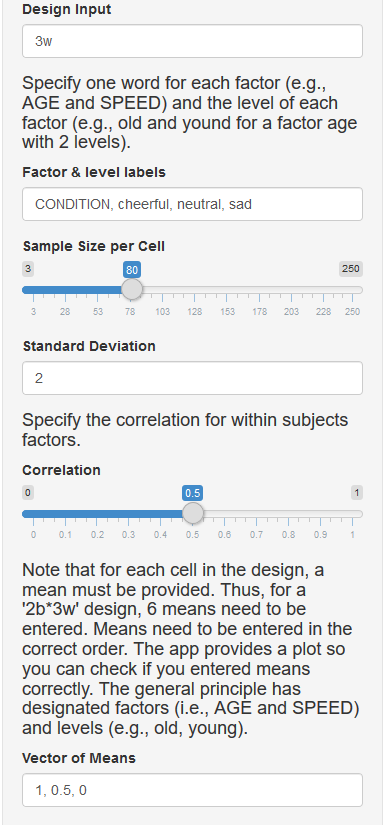
\includegraphics{https://raw.githubusercontent.com/Lakens/ANOVA_power_simulation/master/Appendix/DesignInput_3wSim.PNG}
\caption{}
\end{figure}

This provides the following output in the Shiny app, and we can verify
that the design is entered correctly.

\begin{figure}
\centering
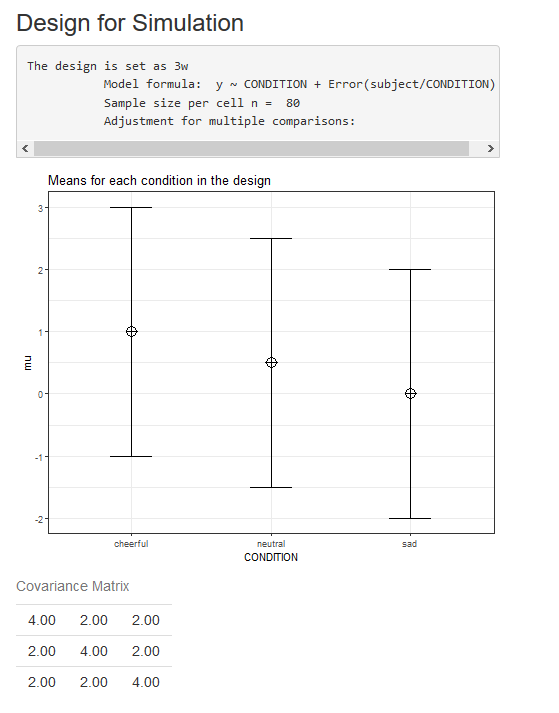
\includegraphics{https://raw.githubusercontent.com/Lakens/ANOVA_power_simulation/master/Appendix/DesignOutput_3wSim.PNG}
\caption{}
\end{figure}

The within-subjects design has been specified; now we run the simulation
with the following information input in the Shiny app.

\begin{figure}
\centering
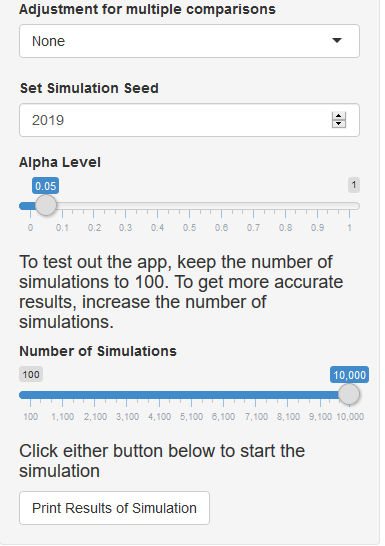
\includegraphics{https://raw.githubusercontent.com/Lakens/ANOVA_power_simulation/master/Appendix/SimInput_3w.PNG}
\caption{}
\end{figure}

This provides the following output.

\begin{figure}
\centering
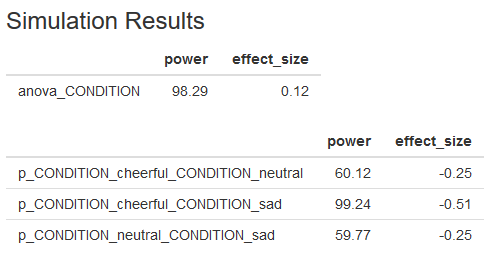
\includegraphics{https://raw.githubusercontent.com/Lakens/ANOVA_power_simulation/master/Appendix/SimResult_3wSim.PNG}
\caption{}
\end{figure}

A Markdown report of the results can be found
\href{https://github.com/Lakens/ANOVA_power_simulation/blob/master/Appendix/Report_3wSim.pdf}{here}.

\section{Power for Interactions: Scenario
\#1}\label{power-for-interactions-scenario-1}

In addition to simple one-way effects, in the manuscript we demonstrate
the power analysis for 2x2 between-subjects design. In this scenario
there two factors ``condition'' and ``voice''. Again, participants are
exposed to a ``sad'' or ``cheerful'' condition. However, the voice is
either human-like (``human'') or robotic (``robot''). Note how we first
specify the factor name for the first factor, then the names for all
levels of the factor, and then specify the second factor label, and the
labels for each level. For the first interaction simulation, we will
also set the sample size to 40 observations per cell.

\begin{figure}
\centering
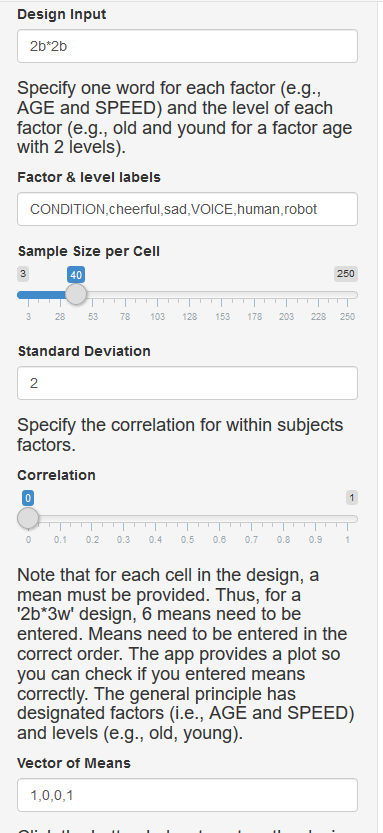
\includegraphics{https://raw.githubusercontent.com/Lakens/ANOVA_power_simulation/master/Appendix/DesignInput_Inter1Sim.PNG}
\caption{}
\end{figure}

This creates the following design output in the Shiny app.

\begin{figure}
\centering
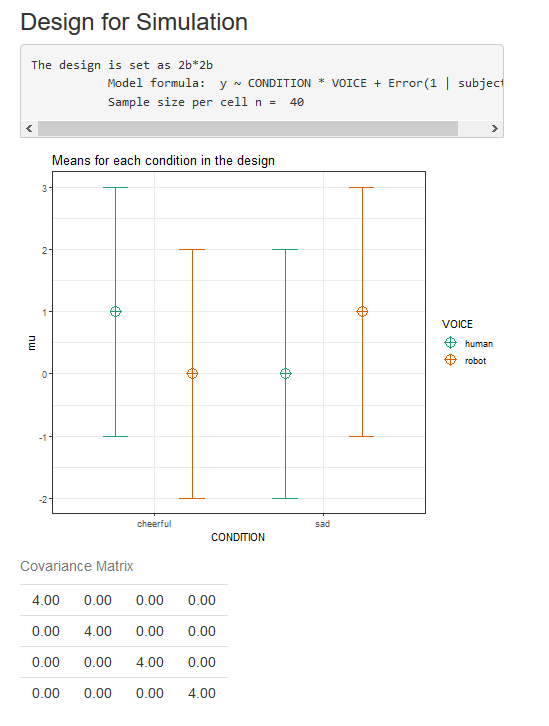
\includegraphics{https://raw.githubusercontent.com/Lakens/ANOVA_power_simulation/master/Appendix/DesignOutput_Inter1Sim.PNG}
\caption{}
\end{figure}

We now can specify the simulation settings.

\begin{figure}
\centering
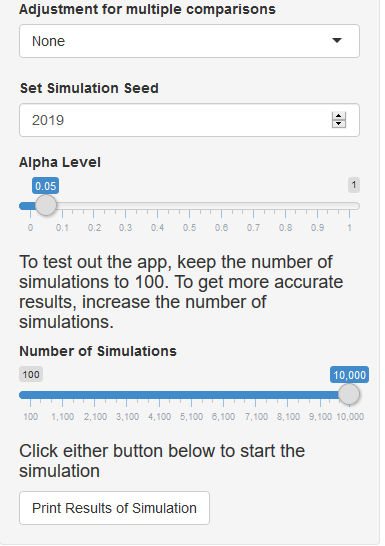
\includegraphics{https://raw.githubusercontent.com/Lakens/ANOVA_power_simulation/master/Appendix/SimInput_3w.PNG}
\caption{}
\end{figure}

Which provides the following results, and a Markdown report can be
downloaded from
\href{https://github.com/Lakens/ANOVA_power_simulation/blob/master/Appendix/Report_3wSim.pdf}{here}.

\begin{figure}
\centering
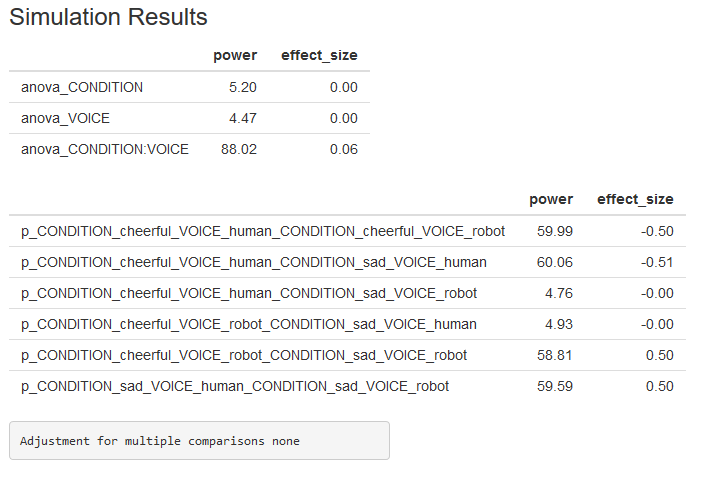
\includegraphics{https://raw.githubusercontent.com/Lakens/ANOVA_power_simulation/master/Appendix/SimResult_Inter1Sim.PNG}
\caption{}
\end{figure}

\section{Power for Interactions: Scenario
\#2}\label{power-for-interactions-scenario-2}

This simulation is almost identical to the previous simulation. The only
difference is the sample size is increased to 80.

The results of the simulation (n = 80) is included below and a Markdown
report can also be downloaded
\href{https://github.com/Lakens/ANOVA_power_simulation/blob/master/Appendix/Report_Inter2.pdf}{here}

\begin{figure}
\centering
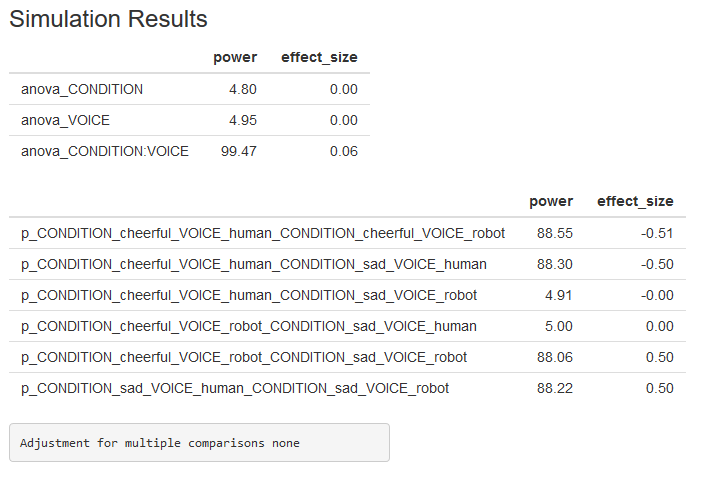
\includegraphics{https://raw.githubusercontent.com/Lakens/ANOVA_power_simulation/master/Appendix/SimResult_Inter2Sim.PNG}
\caption{}
\end{figure}

\section{Power for Multiple
Comparisons}\label{power-for-multiple-comparisons}

As mentioned in the manuscript, the number of pairwise comparisons, if
left unadjusted, can increase the Type I error rate. So in the
manuscript, we revisited the 40 person per group study from the
cross-over interaction example. The design below is the exactly same as
the first scenario presented for interactions (see above). The only
difference in this simulation is that we specify a Holm-Bonferroni
correction for multiple comparisons.

\begin{figure}
\centering
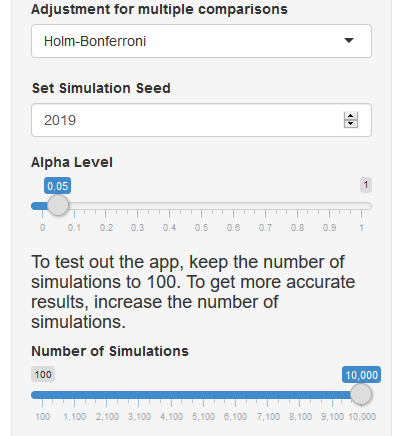
\includegraphics{https://raw.githubusercontent.com/Lakens/ANOVA_power_simulation/master/Appendix/SimInput_Multi.PNG}
\caption{}
\end{figure}

As we can see from this simulation, power for the first pairwise
comparison (cheerful-human vs cheerful-robot) is lower now that the
Holm-Bonferroni (holm) correction is applied.

\begin{figure}
\centering
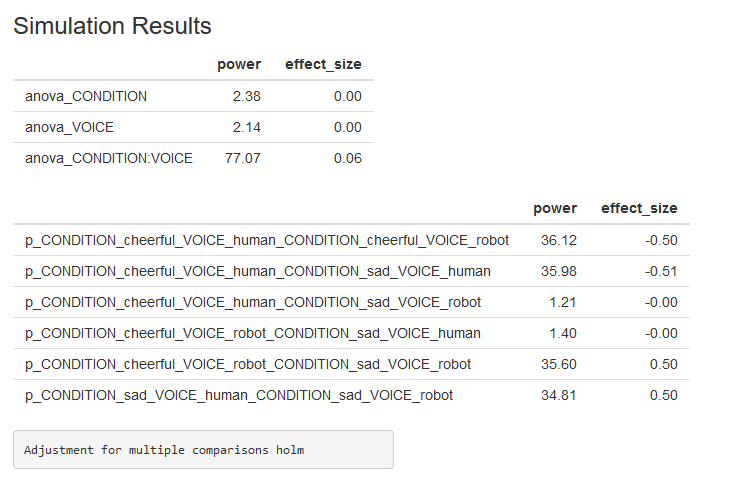
\includegraphics{https://raw.githubusercontent.com/Lakens/ANOVA_power_simulation/master/Appendix/SimResult_MultiSim.PNG}
\caption{}
\end{figure}

The results of this simulation can also be found in a Markdown report
\href{https://github.com/Lakens/ANOVA_power_simulation/blob/master/Appendix/Report_Multi.pdf}{here}.


\end{document}
